\section{Basic operation and their notation}

\exo[Inner/outer products in Dirac notation]

\begin{align*}
\left(\begin{array}{cccc}
 1 &0 \\
\end{array}\right)
\left(\begin{array}{c}
 1\\
 0 \\
\end{array}\right) =
\left(\begin{array}{c}
 1
\end{array}\right)
\quad
\left(\begin{array}{cccc}
 1 &0 \\
\end{array}\right)
\left(\begin{array}{c}
 0\\
 1
\end{array}\right) =
\left(\begin{array}{c}
 0\\
\end{array}\right)
\quad
\left(\begin{array}{cccc}
 1 &2 \\
\end{array}\right)
\left(\begin{array}{c}
 3\\
 4
\end{array}\right) =
\left(\begin{array}{c}
 11
\end{array}\right)
\end{align*}
The last one in Dirac notation :
\begin{align*}
  & (\bra{0} + 2\bra{1}) \times (3\ket 0 + 4 \ket 1) \\
  =& 3\braket 0 0 + 4 \braket 0 1 + 6 \braket 1 0 + 8 \braket 1 1 \\
  =& 3 + 8 \\
  =& 11
\end{align*}
\begin{align*}
\left(\begin{array}{c}
 1\\
 0
\end{array}\right)
\left(\begin{array}{cccc}
 1 &0 \\
\end{array}\right)
=
\left(\begin{array}{cccc}
 1 &0 \\
 0 &0 \\
\end{array}\right)
\qquad
\left(\begin{array}{c}
 0\\
 1
\end{array}\right)
\left(\begin{array}{cccc}
 1 &0 \\
\end{array}\right)
=
\left(\begin{array}{cccc}
 0 &0 \\
 1 &0 \\
\end{array}\right)
\qquad
\left(\begin{array}{c}
 3\\
 4
\end{array}\right)
\left(\begin{array}{cccc}
 1 &2 \\
\end{array}\right)
=
\left(\begin{array}{cccc}
 3 &6 \\
 4 &8 \\
\end{array}\right)
\end{align*}
The last two in Dirac notation :
\begin{align*}
  & (3\ket{0} + 4\ket{1}) \times (\bra 0 + 2\bra 1) \\
  =& 3 \ket 0 \bra 0 + 6 \ket 0 \bra 1 + 4 \ket 1 \bra 0 + 8 \ket 1 \bra 1
\end{align*}

\exo[Matrix products in Dirac notation]
\label{ex1.2:matrix}
\begin{align*}
\left(\begin{array}{cccc}
 0 &0 \\
 1 &0
\end{array}\right)
\left(\begin{array}{c}
 1\\
 0
\end{array}\right)
=
\left(\begin{array}{c}
 0\\
 1
\end{array}\right)
\qquad
\left(\begin{array}{cccc}
 0 &0\\
 1 &0
\end{array}\right)
\left(\begin{array}{c}
 0\\
 1
\end{array}\right)
=
\left(\begin{array}{c}
 0\\
 0
\end{array}\right)
\qquad
\left(\begin{array}{cccc}
 1 &3 \\
 2 &4
\end{array}\right)
\left(\begin{array}{c}
 5\\
 6
\end{array}\right)
=
\left(\begin{array}{c}
 23\\
 34
\end{array}\right)
\end{align*}
The last one in Dirac notation :
\begin{align*}
  &(\ket 0 \bra 0 + 3\ket 0 \bra 1 + 2 \ket 1 \bra 0 + 4 \ket 1 \bra 1)\times
  (5\ket 0 + 6 \ket 1) \\
  =&5\ket 0 \braket 0 0 + 6 \ket 0 \braket 0 1 + 15 \ket 0 \braket 1 0 + 18
    \ket 0 \braket 1 1 + \\
  & 10 \ket 1 \braket 0 0 + 12 \ket 1 \braket 0 1 + 20 \ket 1 \braket 1 0 +
    24 \ket 1 \braket 1 1\\
  =&5 \braket 0 0 \ket 0 + 18 \braket 1 1 \ket 0 + 10 \braket 0 0 \ket 1 +
  24 \braket 1 1 \ket 1 \\
  =&5 \ket 0 + 18 \ket 0 + 10 \ket 1 + 24 \ket 1 \\
  =&23  \ket 0 + 24 \ket 1
\end{align*}

\begin{mathpar}
\left(\begin{array}{cc}
 1& 0\\
 0& 1
\end{array}\right)
\left(\begin{array}{cc}
 1& 3\\
 2& 4
\end{array}\right)
=
\left(\begin{array}{cc}
 1& 3\\
 2& 4
\end{array}\right)
\and
\left(\begin{array}{cc}
 0& 0\\
 0& 1
\end{array}\right)
\left(\begin{array}{cc}
 0& 0\\
 0& 1
\end{array}\right)
=
\left(\begin{array}{cc}
 0& 0\\
 0& 1
\end{array}\right)
\newline
\left(\begin{array}{cc}
 1/\sqrt{2}& 1/\sqrt{2}\\
 1/\sqrt{2}& -1/\sqrt{2}
\end{array}\right)
\left(\begin{array}{cc}
 1/\sqrt{2}& 1/\sqrt{2}\\
 1/\sqrt{2}& -1/\sqrt{2}
\end{array}\right)
=
\left(\begin{array}{cc}
  1& 0\\
  0& 1
\end{array}\right)
\end{mathpar}
The last one in Dirac notation :
\begin{align*}
  &(1/\sqrt 2\ket 0 \bra 0 + 1/\sqrt 2\ket 0 \bra 1 + 1/\sqrt 2 \ket 1 \bra 0
  -1/\sqrt 2 \ket 1 \bra 1)^2 \\
  =& 1/2 \ket 0 \braket 0 0 \bra 0 + 1/2 \ket 0 \braket 0 0 \bra 1 + 1 /2 \ket 0
  \braket 1 1 \bra 0 - 1 / 2 \ket 0 \braket 1 1 \bra 1 \\
  & 1/2 \ket 1 \braket 0 0 \bra 1 + 1/2 \ket 1 \braket 0 0 \bra 0 - 1 /2 \ket 1
  \braket 1 1 \bra 0 + 1 /2 \ket 1 \braket 1 1 \bra 1\\
  =& 1/2 \ket 0 \bra 0 + 1 /2 \ket 0 \bra 0 +
  1/2 \ket 1 \bra 1 + 1 /2 \ket 1 \bra 1\\
  =& \ket 0 \bra 0 + \ket 1 \bra 1
\end{align*}

\newpage
\exo[Tensor products in Dirac/Coecke notation]
\begin{mathpar}
\left(\begin{array}{c}
 1\\
 0
\end{array}\right)
\otimes
\left(\begin{array}{c}
 0\\
 1
\end{array}\right)
=
\left(\begin{array}{c}
 0\\
 1\\
 0\\
 0
\end{array}\right)
\and
\left(\begin{array}{c}
 0\\
 1
\end{array}\right)
\otimes
\left(\begin{array}{c}
 1\\
 0
\end{array}\right)
=
\left(\begin{array}{c}
 0\\
 0\\
 1\\
 0
\end{array}\right)
\and
\left(\begin{array}{c}
 1\\
 2
\end{array}\right)
\otimes
\left(\begin{array}{c}
 3\\
 4
\end{array}\right)
=
\left(\begin{array}{c}
 3\\
 4\\
 6\\
 8
\end{array}\right)\\
\left(\begin{array}{c}
 1\\
 0
\end{array}\right)
\otimes
\left(\begin{array}{c}
 1\\
 0
\end{array}\right)
+
\left(\begin{array}{c}
 0\\
 1
\end{array}\right)
\otimes
\left(\begin{array}{c}
 0\\
 1
\end{array}\right)
=
\left(\begin{array}{c}
 1\\
 0\\
 0\\
 0
\end{array}\right)
+
\left(\begin{array}{c}
 0\\
 0\\
 0\\
 1
\end{array}\right)
=
\left(\begin{array}{c}
 1\\
 0\\
 0\\
 1
\end{array}\right)
\end{mathpar}
The last two in Dirac notation :
\begin{align*}
  (\ket 0 + 2 \ket 1) \otimes (3 \ket 0 + 4 \ket 1)
  =& 3 \ket{00} + 4 \ket{01} + 6 \ket{10} + 8 \ket{11}
\end{align*}
\begin{align*}
  \ket 0 \otimes \ket 0 + \ket 1 \otimes \ket 1
  =& \ket{00} + \ket{11}
\end{align*}

\begin{mathpar}
\left(\begin{array}{cc}
 1&0\\
 0&1
\end{array}\right)
\otimes
\left(\begin{array}{cc}
 1&0\\
 0&1
\end{array}\right)
=
\left(\begin{array}{cccc}
  1&0&0&0\\
  0&1&0&0\\
  0&0&1&0\\
  0&0&0&1
\end{array}\right)
\and
\left(\begin{array}{cc}
 1&0\\
 0&0
\end{array}\right)
\otimes
\left(\begin{array}{cc}
 1&0\\
 0&1
\end{array}\right)
=
\left(\begin{array}{cccc}
  1&0&0&0\\
  0&1&0&0\\
  0&0&0&0\\
  0&0&0&0
\end{array}\right)
\\
\left(\begin{array}{cc}
 1/\sqrt{2}& 1/\sqrt{2}\\
 1/\sqrt{2}& -1/\sqrt{2}
\end{array}\right)
\otimes
\left(\begin{array}{cc}
 1/\sqrt{2}& 1/\sqrt{2}\\
 1/\sqrt{2}& -1/\sqrt{2}
\end{array}\right)
=
\left(\begin{array}{cccc}
  1/2& 1/2& 1/2& 1/2\\
  1/2&-1/2& 1/2&-1/2\\
  1/2& 1/2&-1/2&-1/2\\
  1/2&-1/2&-1/2& 1/2
\end{array}\right)
\end{mathpar}

In Dirac notation :

\begin{align*}
  &(\ket 0 \bra 0 + \ket 1 \bra 1) \otimes (\ket 0 \bra 0 + \ket 1 \bra 1) \\
  =& \ket 0 \bra 0 \otimes \ket 0 \bra 0 + \ket 0 \bra 0 \otimes \ket 1 \bra 1 +
  \ket 1 \bra 1 \otimes \ket 0 \bra 0 + \ket 1 \bra 1 \otimes \ket 1 \bra 1 \\
  =& \ket 0 \bra 0 + \ket 1 \bra 1 + \ket 2 \bra 2 +\ket 3 \bra 3
\end{align*}
\begin{align*}
  &(\ket 0 \bra 0) \otimes (\ket 0 \bra 0 + \ket 1 \bra 1) \\
  =& \ket 0 \bra 0 \otimes \ket 0 \bra 0 + \ket 0 \bra 0 \otimes \ket 1 \bra 1
  \\
  =& \ket 0 \bra 0 + \ket 1 \bra 1
\end{align*}
\begin{align*}
  1/\sqrt 2  (&\ket 0 \bra 0 + \ket 0 \bra 1 + \ket 1 \bra 0 - \ket 1 \bra 1 )
    \otimes 1/\sqrt 2 (\ket 0 \bra 0 + \ket 1 \bra 0 + \ket 1 \bra 0 - \ket 1
    \bra 1) \\
  =1/2 (&\ket 0 \bra 0 + \ket 0 \bra 1 + \ket 0 \bra 2 + \ket 0 \bra 3 + \\
   &\ket 1 \bra 0 - \ket 1 \bra 1 + \ket 1 \bra 2 - \ket 1 \bra 3 + \\
   &\ket 2 \bra 0 + \ket 2 \bra 1 - \ket 2 \bra 2 - \ket 2 \bra 3 + \\
   &\ket 3 \bra 0 - \ket 3 \bra 1 - \ket 3 \bra 2 + \ket 3 \bra 3)
\end{align*}

\newpage

We want to prove $(A \otimes B) (C \otimes D) = (AC) \otimes (BD)$

\begin{itemize}
  \item Dirac's notation :
    
    We have $A = \sum_{i,j} a_{i,j} \ket i \bra j$ and $D = \sum_{k, l}
    d_{k,l}\ket k \bra l$
    \begin{align*}
      (A \otimes B) (C \otimes D)
      &= ((\sum_{i,j} a_{i,j} \ket i \bra j) \otimes B)
         (C \otimes (\sum_{k, l} d_{k,l}\ket k \bra j)) \\
      &= (\sum_{i,j} a_{i,j} \ket i \bra j)C \otimes
         B (\sum_{k, l} d_{k,l}\ket k \bra j) & \text{bilinearity of $\otimes$}\\
      &= (AC) \otimes (BD)
    \end{align*}

  \item Coecke's notation :

    \begin{center}
    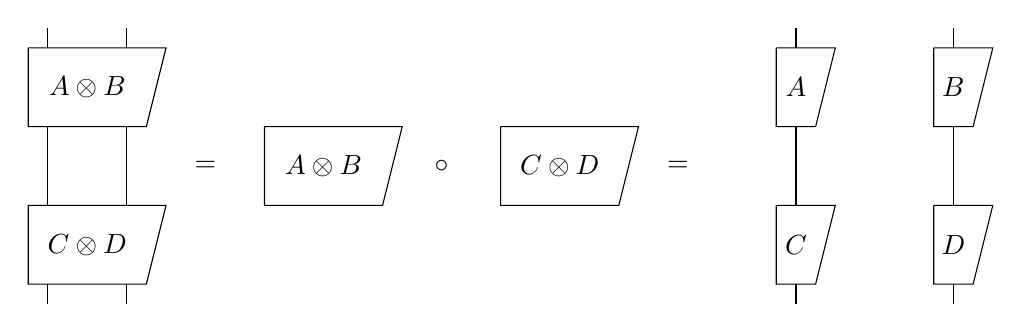
\begin{tikzpicture}
      \node(AB) at (0, 0) {$A \otimes B$};
      \draw (-0.75, 0.5) -- (1, 0.5) -- (0.75, -0.5) -- (-0.75, -0.5) --
            (-0.75, 0.5);
      \node(CD) at (0, -2) {$C \otimes D$};
      \draw (-0.75, -1.5) -- (1, -1.5) -- (0.75, -2.5) -- (-0.75, -2.5) --
            (-0.75, -1.5);

      \draw (-0.5, 0.75) -- (-0.5, 0.5 );
      \draw ( 0.5, 0.75) -- ( 0.5, 0.5 );
      \draw (-0.5,-0.5 ) -- (-0.5,-1.5 );
      \draw ( 0.5,-0.5 ) -- ( 0.5,-1.5 );
      \draw (-0.5,-2.5 ) -- (-0.5,-2.75);
      \draw ( 0.5,-2.5 ) -- ( 0.5,-2.75);

      \node at (1.5, -1) {$=$};

      \node(AB) at (3, -1) {$A \otimes B$};
      \draw (2.25,-0.5) -- (4, -0.5) -- (3.75, -1.5) -- (2.25, -1.5) --
            (2.25,-0.5);
      \node at (4.5, -1) {$\circ$};
      \node(CD) at (6, -1) {$C \otimes D$};
      \draw (5.25,-0.5) -- (7, -0.5) -- (6.75, -1.5) -- (5.25, -1.5) --
            (5.25,-0.5);

      \node at (7.5, -1) {$=$};
      \node(A) at (9, 0) {$A$};
      \draw (8.75, 0.5) -- (9.5, 0.5) -- (9.25, -0.5) -- (8.75, -0.5) --
            (8.75, 0.5);
      \node(B) at (11, 0) {$B$};
      \draw (10.75, 0.5) -- (11.5, 0.5) -- (11.25, -0.5) -- (10.75, -0.5) --
            (10.75, 0.5);
      \node(C) at (9,-2) {$C$};
      \draw (8.75,-1.5) -- (9.5,-1.5) -- (9.25, -2.5) -- (8.75, -2.5) --
            (8.75,-1.5);
      \node(D) at (11,-2) {$D$};
      \draw (10.75,-1.5) -- (11.5,-1.5) -- (11.25, -2.5) -- (10.75, -2.5) --
            (10.75,-1.5);

      \draw (9, 0.75) --  (9, 0.5 );
      \draw (11, 0.75) -- (11, 0.5 );
      \draw (9,-0.5 ) --  (9,-1.5 );
      \draw (11,-0.5 ) -- (11,-1.5 );
      \draw (9,-2.5 ) --  (9,-2.75);
      \draw (11,-2.5 ) -- (11,-2.75);
    \end{tikzpicture}
    \end{center}

\end{itemize}

\exo[Dagger in Dirac/Coecke notation]

\begin{align*}
\left(\begin{array}{cc}
 1/\sqrt{2}& 1/\sqrt{2}\\
 1/\sqrt{2}& -1/\sqrt{2}
\end{array}\right)^\dagger
=
\left(\begin{array}{cc}
 1/\sqrt{2}& 1/\sqrt{2}\\
 1/\sqrt{2}& -1/\sqrt{2}
\end{array}\right)
\qquad
\left(\begin{array}{cc}
 1& 3i\\
 2& 4i
\end{array}\right)^\dagger
=
\left(\begin{array}{cc}
 1& 2\\
 -3i& -4i
\end{array}\right)
\end{align*}
In Dirac notation:
\begin{align*}
  &1/\sqrt 2 (\ket 0 \bra 0 + \ket 0 \bra 1 + \ket 1 \bra 0 - \ket 1 \bra
    1)^\dagger \\
  =&1/\sqrt 2 (\ket 0 \bra 0 + \ket 1 \bra 0 + \ket 0 \bra 1 - \ket 1 \bra 1)
\end{align*}
\begin{align*}
  &(\ket 0 \bra 0 + 3i \ket 0 \bra 1 + 2 \ket 1 \bra 0 + 4i \ket 1 \bra
    1)^\dagger \\
  =&(\ket 0 \bra 0 - 3i \ket 1 \bra 0 + 2 \ket 0 \bra 1 - 4i \ket 1 \bra
    1)
\end{align*}

\exo[Gates in Dirac notations]

$$ H = 1/\sqrt 2 (\ket 0 \bra 0+\ket 0 \bra 1+\ket 1 \bra 0-\ket 1 \bra 1)$$
$$ \textit{CNot} = \ket 0 \bra 0+\ket 1 \bra 1+\ket 3 \bra 2+\ket 2 \bra 3$$
$$ T = \ket 0 \bra 0 + e^{\frac{i\pi}{4}} \ket 1 \bra 1$$

Proof that are unitary matrix :

\begin{itemize}
  \item $H$ : $H^\dagger H = Id_1$ already do in Exercie-\ref{ex1.2:matrix}
  \item \CNot :
    \begin{align*}
      \CNot^\dagger \CNot &= 
        (\ket 0 \bra 0+\ket 1 \bra 1+\ket 3 \bra 2+\ket 2 \bra 3)
        (\ket 0 \bra 0+\ket 1 \bra 1+\ket 2 \bra 3+\ket 3 \bra 2) \\
        &=(\ket 0 \bra 0 + \ket 1 \bra 1 + \ket 2 \bra 2 + \ket 3 \bra 3) \\
        &= Id_4
    \end{align*}
  \item $T$:
    \begin{align*}
      &(\ket 0 \bra 0 + e^{\frac{i\pi}{4}} \ket 1 \bra 1)
       (\ket 0 \bra 0 + e^{\frac{-i\pi}{4}} \ket 1 \bra 1) \\
      =& \ket 0 \braket 0 0 \bra 0 + e^{\frac{i\pi}{4}} \ket 0 \braket 0 1 \bra 1
          + e^{\frac{i\pi}{4}}(\ket 1 \braket 1 0 \bra 0)
          + e^{\frac{i\pi}{2}}(\ket 1 \braket 1 1 \bra 1)\\
      =& \ket 0 \bra 0 + \ket 1 \bra 1
    \end{align*}
\end{itemize}

\exo[Pauli matrices in Dirac/Coecke notation]~

\begin{itemize}
  \item For all $i, k \in [0, 3]$ we want to show
    $\sigma_i \sigma_j = \delta_{ij} I + i \sum_k \epsilon_{ijk} \sigma_k$

    \begin{itemize}
      \item If $i=j$ then $\sigma_i \sigma_j = I$ and for all $k$ we have
        $\epsilon_{ijk} = 0$.

        So we have $\delta_{ij} I = I = \sigma_i \sigma_j$
      \item If $j = i + 1$
    \end{itemize}

  \item For all $i, k \in [0, 3]$ we want to show $[\sigma_i, \sigma_j] = 
    2i \sum_k \epsilon_{ijk}$
    \begin{align*}
      [\sigma_i, \sigma_j] &= \sigma_i \sigma_j - \sigma_i \sigma_j \\
      &= (\delta_{ij} I + i \sum_k \epsilon_{ijk} \sigma_k) -
         (\delta_{ji} I + i \sum_k \epsilon_{jik} \sigma_k) \\
      &= i \sum_k \epsilon_{ijk} \sigma_k - i \sum_k \epsilon_{jik} \sigma_k \\
      &= i \sum_k \epsilon_{ijk} \sigma_k + i \sum_k \epsilon_{ijk} \sigma_k \\
      &= 2i \sum_k \epsilon_{ijk} \sigma_k
    \end{align*}
  \item For all $i, k \in [0, 3]$ with $i\not = j$ we want to show $\{\sigma_i, \sigma_j\} = 0$
    \begin{align*}
      \{\sigma_i, \sigma_j\} &= \sigma_i \sigma_j + \sigma_i \sigma_j \\
      &= \delta_{ij} I + i \sum_k \epsilon_{ijk} \sigma_k +
         \delta_{ji} I - i \sum_k \epsilon_{ijk} \sigma_k & \epsilon_{jik} =
         -\epsilon_{ijk}\\
      &= 2 \delta_{ij} I \\
      &= 0 & i \not = j
    \end{align*}
\end{itemize}


